\documentclass[sigconf,edbt]{acmart-edbt2021}

\def\BibTeX{{\rm B\kern-.05em{\sc i\kern-.025em b}\kern-.08em
    T\kern-.1667em\lower.7ex\hbox{E}\kern-.125emX}}

\usepackage{booktabs} % For formal tables

\setcopyright{none}
\renewcommand\footnotetextcopyrightpermission[1]{}


\settopmatter{printacmref=false, printccs=false, printfolios=false}

\pagestyle{empty} % removes running headers


\begin{document}
\title{Data Mining project}
\subtitle{Recommendation system for Medical Environment}
  

\author{Bertelli Davide\\Artificial Intelligence Systems, $2^{nd}$ year.}
\affiliation{%
  \institution{University of Trento}
  \streetaddress{Via Sommarive 9, Povo}
  \city{Trento} 
  \state{Italy} 
  \postcode{38123}
}
\email{bertellidavide98@gmail.com}

% The default list of authors is too long for headers}
% \renewcommand{\shortauthors}{B. Trovato et al.}
% \renewcommand{\shortauthors}{}


\begin{abstract}
This report provides the algorithms, formulations and code implementations that
allowed to build a recommendation system applicable to the medical environment.
The algorithm leveraged on the biological similarity among the known patients
to provide its suggestions.
The system implemented is an hybrid one which uses a content-based rating
method as a baseline for its ratings and improves them through a collaborative
filtering algorithm.
The results of the system had been evaluated using the RMSE scoring strategy
over datasets containing different numbers of available patients, and leading
to an average RMSE value of 0.31.
\end{abstract}


\maketitle

\section{Introduction and Motivation}
In a medical environment a patient asks for suggestions to a
doctor regarding one or more diseases it is suffering from. Usually the
therapies suggested came from the doctor own experience.
In this perspective, the personal experience covers the highest importance in
formulating a diagnosis of the disease and healing the patient.
Given this environment it was thought to provide suggestions for a specific 
condition using as experience a dataset filled with the medical history of
several patients.
A good recommendation system for this scenario could serve as an artificial 
collegue for the medical staff or as a tool to allow the patients'
self-treatment for the most common diseases, even though a professional
opinion must be always required.
What has been tried to achieve with this work is a Recommendation System able
to suggest the best therapies to which a patient should undergo to
cure a specific disease it is suffering from. To perform those
suggestions the system must know the medical
history of some patients, to use as experience, and the one of the patient
under analysis, together with a list of therapies that may be suggested. 

\section{Related Work}
\subsection{Recommendation Systems}
The recommendation systems field is very extended, anyway it is possible to
classify the available algorithms in three main categories:
% https://towardsdatascience.com/recommendation-systems-explained-a42fc60591ed
\begin{enumerate}
		\item The \textbf{Content-based Recommendation Systems} which work by 
		      providing suggestions based on the user's previous ratings for
			  objects similar to the one to suggest. It has a dual
			  implementation depending on which
			  elment it is more focused on. If more attention is 
			  given to the items available then the recommendation system will
			  be an item-profile one, otherwise if users are more relevant for
			  the final application it will be a user-profile one.
			  % Maybe put the advantages ?
		\item The \textbf{Collaborative Filtering Recommendation Systems} which
		      works
		      by leveraging on the ratings of an object coming from several
		      users. The idea behind this agorithm is that two 
			  users that have a similar taste may like a specific object in the
			  same way.
			  This system splits into two kinds: the model based and the
			  memory based. The first exploits machine learning techniques
			  for predicting the ratings, the latter uses the
			  "neighbours" of the user-item combination under analysis to
			  provide a prediction and it is further divided into item and
			  user based collaborative filtering depending on which element to
			  focus on.
			  % Maybe put the advantages ?
		\item The \textbf{Hybrid Recommendation Systems} are systems designed
		      to provide more robust predictions merging methods of the
			  previous categories or, even, combining their results.
			  % Maybe put the advantages ?
\end{enumerate}
Independently by its category, a Recommendation System, reaches a suggestion
identifying which objects, users or items, are similar to the one under
analysis or to the ones for which the ratings are available.
\subsection{Similarity Scores}
The similarity
is a mathematical score that is attributed to pairs of objects. Its 
computation can be performed through different metrics such as:
\begin{itemize}
		\item The \textbf{Jaccard Similarity} which is defined as the ratio
		      of the intersection with the union. Meaning that two objects are
			  similar if they have a lot of elements in common.
			  \begin{equation}
				\frac{|obj_{1} \bigcap obj_{2}|}{|obj_{1} \bigcup obj_{2}|}
			  \end{equation}
			  Where $obj_{i}$ represents the ratings vector for a specific
			  object.
		\item The \textbf{Euclidean Distance} which defines that two objects
		      are similar if they are close to each other.
			  \begin{equation}
				d = \sqrt{(obj_{1,1}-obj_{2,1})^{2} + \dots +
						  (obj_{1,N}-obj_{2,N})^{2}}
			  \end{equation}
			  Where $obj_{i, j}$ represents the $j^th$ rating of object $i$,
			  Supposing that $obj_{1}$ and $obj_{2}$ are the ratings vectors
			  associated to an object in an $N$ dimensional space of users or
			  items.
		\item The \textbf{Cosine similarity} which works by measuring the
		      amplitude of the angle between the ratings vectors associated to
			  two objects.
		      The lesser the amplitude, the higher the similarity.
			  \begin{equation}
				cos_{simm} = cos(obj_{1}, obj_{2})
						   = \frac{obj_{1}*obj_{2}}{\|obj_{1}\|\|obj_{2}\|}
			  \end{equation}
			  Where $obj_{i}$ are the ratings vectors for some objects in the
			  $N$ dimensional space of user or items.

			  It exist a slight variation called 
			  \textbf{Centered Cosine Similarity} which is the same as defined
			  above, but the vectors are previously normalized by subtracting
			  their own mean.
\end{itemize}
\subsection{Evaluation Metrics}
Lastly, the Recommendation Systems need a tool able to measure their
performances and to allow an objective comparison among different
implementations. Some of the most used evaluation metrics are:
\begin{itemize}
		\item The \textbf{K-fold} which works by splitting the data available into
		      random subsets, folds, which will be used for training and testing:
			  specifically k-1 for training and the left one for testing.
			  The testing is performed many
			  times with different folds and at the end the mean accuracy is
			  computed as the average score of the system performances.
		\item The \textbf{Mean Squared Error MSE} is a metric computed by
		      averaging the error occured between the predicted ratings and
			  their true values. It exist a variation called
			  \textbf{Root Mean Squared Error} which is the square root of the
			  MSE.
			  \begin{equation}
				MSE = \frac{\sum_{t\in Test}|r_{t}-r_{t}^{*}|}{|Test|} \quad 
				RMSE= \sqrt{MSE}
			  \end{equation}
				With $r_{t}$ and $r_{t}^{*}$ being the truth and predicted
				values, while $|Test|$ is the number of elements under testing.
\end{itemize}
\subsection{Project Setup}
In this work it has been built an Hybrid Recommendation System using
the global baseline estimate method of the Content Based Recommendation
Systems, to improve the prediction performances of a Collaborative Filtering
one.
The system built uses the euclidean distance to compute the similarity among
the objects and it has been evaluated using the RMSE metric.

\section{Problem Statement}
Supposing an input dataset $D$ composed of the recorded medical histories of
some patients $D_P$, a set of known condition, $D_C$, and a set of available
therapies $D_T$
\begin{equation}
		D = D_P \cup D_T \cup D_C
\end{equation}
the problem of suggesting the best therapies for a condition $c$ to a patient
$P_q$ can be formally expressed in finding a utility function $u$ such as:
% \begin{equation}
% 		u: \quad (P_{q}^{t}|_{c} \cup P^{t}|_{c}) \times D_{t} \to r_{t|_c}
% \end{equation}
% Where $P_{q}^{t}|_{c}$ and $P^{t}|_{c}$ are, respectively, the set of
% therapies already tried by the query patient $P_q$ and other patients $P$ given
% the specific condition $c$. $D_{t}$ is the set of therapies which are known to
% the system and contained in the dataset. $r_{t|_c}$ is the rating of a certain
% therapy $t$ for a specific query condition $c$.
\begin{equation}
		u: (P_{q}|_{c} \cup D_{P}|_{c}) \times D_{T} \to r_{t}|_{c}
        \quad t \in \{D_{T}\setminus\{P^{T}_{q}|_{c}\}\}
\end{equation}
Where: $P_{q}|_{c}$ is the set of rating scores for therapies that the patient
$P_q$, the query patient, has already tried for healing itself from
the condition $c$;
$D_{P}|_{c}$ is the set of rating scores for the therapies that the patients in
the dataset have tried for the condition $c$;
$D_{T}$ is the set of therapies available in the dataset;
$P^{T}_{q}|_{c}$ is the set of therapies that have already been tried by the
query patient;
$r_{t}|_{c}$ is the rating of a therapy $t$ for a condition $c$.
\section{Solution}
The solution provided in this report, works as follows.
Given in input the query patient $P_q$ and the condition $c$ for which the
suggestions have to be made, a utility matrix $u_c$ is built parsing
the medical history of all the patients in the given dataset, $D_{P}$, and
retaining the rating scores of the therapies for those patients that underwent
the specific condition.
\begin{equation}
		u_c : \{P_{i}|_{c}\} \quad
		\forall P_i :P_i \in \{D_{P}|_{c} \cup P_{q}|_{c}\}
\end{equation}
\begin{equation}
		u_c =
		\begin{bmatrix}
				r_{1,1} & r_{1,2} & \dots & r_{1,j} \\ 
				r_{2,1} & r_{2,2} & \dots & r_{2,j} \\ 
				\vdots & \vdots & \vdots & \vdots \\
				r_{i,1} & r_{i,2} & \dots & r_{i,j} 
		\end{bmatrix}
		\substack{i \in \{D_{P}|_{c}\} \\ j \in \{D_T\}}
\end{equation}
Where $P_i|_{c}$ is the ratings vector of therapies that the patients in the
dataset underwent in order to get cured by the condition $c$;
$D_{P}|_{c}$ is a subset of the input dataset containing the ratings of
therapies for those patients which have been subjected to the condition $c$;
$P_q|_{c}$ is the ratings vector for the therapies already tried by the
query patient for the condition $c$;
$r_{i,j}$ is the rating provided by the $i^{th}$ patient to the $j^{th}$
therapy, i.e. the rate of success. \newline
Once the matrix is built, each rating vector in it undergo a
weighting process dependent by its average goodness across the patients that
used it:
\begin{equation}
		r_{i,j} = \Bigg (\frac{\sum_{i \in D_{P}|_{c}} r_{i,j}}
							  {R_{j}*100}\Bigg) * r_{i,j}	
		\quad
		\forall j \in D_T
\end{equation}
Where $R_{j}$ is the number of elements in the $j^{th}$ therapy ratings
vector.
Then, the patient vectors are centered with respect to 0 by subtracting their
mean value, in order to make all the scores comparable:
\begin{equation}
		r_{i, j} = r_{i, j} - \Bigg(\frac{\sum_{j \in D_T} r_{i,j}}
							  {R_{i}}\Bigg)
		\quad
		\forall i \in D_{P}|c
\end{equation}
Where $R_{i}$ is the number of elements in the $i^{th}$ patient ratings
vector.
Lastly, a normalization is performed in order to enforce the maximum value
in the matrix to be 1.
\begin{equation}
		r_{i,j} = \frac{r_{i,j}}{max(u_t)}
		\quad \forall i \in D_{P}|c
		\quad \forall j \in D_T
\end{equation}
% Line 869
After the normalization steps, the query patient's ratings vector is removed
from the utility matrix and it is used to find the most similar patients.
As anticipated in section 2 the euclidean distance(2) is used to compute the
similarity between patients and the most similar ones are identified by being
the closest to the query patient.
This metric is used instead of the cosine similarity due to
the high sparsity of the utility matrix which negatively affected the
computation of the cosine.
To perform the computation of the distance, the empty cells of the matrix
have been temporary filled with a 0 value.
The nearest neighbours are identified as the patients within a distance less than
half the length of the query patient vector.
To further improve the similarity it has been thought to increase the 
similarity score for those patients which have a similar biology to
the query one, as described in section 5.3.
Then, for the patients found,  their similarity
score was risen in order to contribute more in the ratings prediction
computation. Due to the usage of the euclidean distance, increase the
similarity means to reduce the distance and so a -1 value was added to the
similarity score of the patients having the same biology of the query one.
%Line 992
Having found the nearest neighbours set, the
prediction of the ratings for the therapies not tried by the query patient
begins. Specifically, it is possible to define the rating of
a therapy $t$ for the query patient $P_q$ as:
\begin{equation}
		r_{P_q, t} = b_{P_q,t} + \frac{\sum_{i \in NN}|1-S_{P_q,i}|(r_{i,t}-b_{i,t})}
								  {\sum_{i \in NN}|1-S_{P_q,i}|}
\end{equation}
% Rating of patient p over therapy t
Where $S_{p,i}$ is the similarity score between the query patient ratings
vector and the ratings vector of the $i^{th}$ patient in the Nearest Neighbours
set $NN$. $r_{i, t}$ is the rating of the therapy $t$ attributed by the
$i^{th}$ patient in the Nearest Neighbour set. $b_{p,t}$ and $b_{i, t}$ are the
baseline estimates inherited by the Content based Recommendation systems.
Their computation is performed using the following equations:
%Line 965
\begin{equation}
		b_{p,t} = mean(u_c) + b_p + b_t
\end{equation}
\begin{equation}
		b_{p} = mean(P_{q}|_{c}) - mean(u_c)
\end{equation}
\begin{equation}
		b_{t} = mean(u_{c}^{t}) - mean(u_c)
\end{equation}
Where $mean(u_c)$ is the mean value of the utility matrix, $mean(P_{q}|_{c})$ is
the mean value of the ratings vector of the query patient and $mean(u_{c}^{t})$
is the mean value of the therapy given its ratings for each patient.
It is important to notice the $|1-S_{P_q,i}|$ in the computations which is due
to the employment of the euclidean distance as the similarity metric.
% *= -1 Maybe is not needed at line 1053
At the end of the computation the ratings vector of the query patient is
completely filled with the estimates and the five highest scoring therapies,
that have not already tried, are used as suggestions.
\section{Implementation}
\subsection{Code Implementation}
The Recommendation System has been written in python 3.8.10 and uses the
pandas module\cite{Pandas} to manage the matrices and vectors.
Custom data structures have been created to represent and better manage the
data coming from the input dataset.
The structures in use are:
\begin{itemize}
		\item The \textbf{Entity} class which is used as the main structure
		      which will be inherited by some of the others classes. It
		      contains an identifier, a name and an optional type field.
		\item The \textbf{Condition} class which inherits the Entity one and
				is used to store the data necessary to represent a Condition
				in the dataset.
		\item The \textbf{Therapy} class which inherits the Entity one and
				is used to represent the data identifying a therapy in the 
				dataset.
		\item The \textbf{Trial} class is the one used to represent a
				trial that a patient has done in order to heal itself from a
				disease. It contains a unique identifier, the begin and end 
				dates of the trial, the condition identifier for which the
				trial was done and the rate of success.
		\item The \textbf{PCondition} class is the one used to store the
				data regarding the conditions affecting the patients. It
				contains its identifier, the diagnosed and cured dates
				and the identifier of the condition in the dataset.
		\item The \textbf{Patient} class which inherits the entity class and is
				used to manage the data representing the patients' medical
				history.
				Specifically, each patient is represented by a name
				in the format "name surname", an identifier
				and two lists: one containing the diseases that
				the patient have been subjected to and the other containing
				the trials done for each of them. This class is especially
				used to represent the medical history of each patient.
		\item The \textbf{Dataset} class is the one used to represent the
				entire input dataset exploiting the classes defined so far.
				It is comprehensive of three lists representing the conditions
				or diseases, known from the input data, the therapies available
				in the dataset and the medical histories of the available
				patients.
				This class contains also the method which generates the utility
				matrix that will be further used to recommend the therapies.
\end{itemize}
\subsection{Utility Matrix Construction}
The utility matrix that is generated by the Dataset
class is built creating a pandas.DataFrame object which rows and columns are
respectively the patients and therapies identifiers gathered from the available
objects in the Dataset class.
Each cell of the matrix is filled by each rating that a patient gave for
the therapies it tried.
If a patient did not underwent a therapy and so there is not any rating
available the NaN value is used as score.
After the building task, a preprocessing step is performed in order to remove
the columns, i.e. the therapies, without scores due to the inability to produce
any rating for a therapy without anyone having used it.
\subsection{Nearest Neighbours Computation}
Then the utility matrix, exploiting the supported operations among the pandas
objects, is subjected to the normalization operations described by the
equations (9), (10) and (11).
After the normalization steps the nearest neighbours of the query patients are
computed using the euclidean distance (2) and saved into a DataFrame. Then 
each patient scorings vector in the utility matrix is filtered over the
therapies that the query patient underwent and the scores are compared. If
a match, with a 10\% tolerance, is found, the patient is said to have
a similar biology to the one of the query patient and its index is saved in a set.
At this point the set of nearest neighbours patients is intersected with the
one containing the indexes of patients having a similar biology.
If the intersection is not empty the patients resulting from it have
their euclidean distance decreased by 1 increasing the similarity and so
giving more weight to their ratings during the prediction step.
\subsection{Ratings Prediction}
As already stated in section 4 the ratings prediction follows the equations
(12), (13), (14) and (15) by exploiting the operations defined for the
pandas objects.
Once the ratings vector for the query patient is completely filled with
the predictions, the therapies that it already tried for the codition under
analysis are removed and the 5 highest scoring therapies are returned to the
user inside a DataFrame object reporting the identifier, name, type and score
of each selected therapy.
\section{Dataset}
The datasets used in the computations is randomly generated.
It contains a fixed set of diseases and therapies plus a variable number of
patients' medical histories.
\subsection{Conditions and Therapies creation}
The conditions and therapies available are taken directly from the internet
by parsing two web pages\cite{ThPool}\cite{CPool} from which the names of the
conditions and therapies are taken, while their types are inferred directly
from the name. Once the couples name-type are generated, a new instance of the
Condition or Therapy class is created and saved into two lists working as pools.
\subsection{Patient Creation}
The patient creation followed a completely different process:
firstly, the names and surnames used for the \emph{name} field have been
sampled through the code made available by a
github repository\cite{NamePool} which returned the most common names and
surnames across the world. These were saved into two lists working as pools.
Having at disposal also the pools for the therapies and conditions, a
user-defined number of patients are created.
After randomly sampling the names and surnames a unique identifier is generated.
Then a randomly chosen number, between 0 and 10, is used to define the
number of diseases in the medical history of the patient and for each of
them the diagnosed and cured date are randomly generated.
Each date is chosen by randomly sampling inside a precise interval,
specifically the diagnosed date is sampled among the birth and death dates 
of the patient: the first is randomly chosen in an interval of 100 years going
from the local date up to the past, the latter is generated by sampling a date
in the interval going from the diagnosed date up to the death date which is
a randomly chosen date computed by subtracting the randomly chosen age of the
patient from 100(the expected human lifespan).
The cured date is the only one allowed to be null, meaning that the disease
is still not healed. Each condition has a probability of 20\% to not being
cured.
After that, for each condition that the patient has, a random number of trials,
between 0 and 10, is generated by randomly sampling the therapies to use from the
respective pool. The dates of start and end of the treatments are chosen in the
same way of the diagnosed and cured one, the only precaution taken is that
for the same condition the trials have to be executed in a subsequent way.

\section{Experimental Evaluation}
The recommendation system has been evaluated in terms of the Root Mean Squared
Error(4) and the time it needs to generate a recommendation.
The system has been built in a way that allows the user to provide the datasets
used for evaluation or even resort to an automatic evaluation
letting the code to generate the datasets. In this latter case the
evaluation is run over four datasets containing different batches of patients:
25, 50, 100 and 150 thousands, while the number of conditions and therapies
available are kept equal in all of them.
The building of the random datasets follows the steps presented in section 6.
% Evaluation steps
Once the recommendation system has a list of datasets on which to work on,
all of them are evaluated sequentially for a certain number of iterations
defined by the user. In my experiments 30 iterations were used.
The evaluation function firstly loads the datasets and saves their values
inside the Dataset class, then
it randomly choses a condition from the one saved in the class and uses it to
build the utility matrix. At this point it randomly samples from the indexes
of the matrix a patient which has tried at least one therapy to cure
the condition. Once the patient is chosen, a therapy is randomly sampled
from the ones the patient underwent and the score of success is saved as the
truth value,
and it is substituted with an \emph{NaN} value to allow the rating function to
work properly. At this point, the nearest neighbours are computed and used
together with the utility matrix, without the selected therapy value, to 
compute the ratings for the chosen therapy. Lastly the predicted value of
the therapy and its real value are subjected to the RMSE computation(4)
ending the first part of the evaluation process.
The RMSE scores across the different iterations are collected and their mean
value is used as the final RMSE score.
% Time evaluation
During those steps the time requested by the algorithm to build the utility
matrix, compute the nearest neighbours and predict the ratings for the therapy
is collected and their mean is used as the final time score.
% Professor and student datasets evaluation
The first evaluation of the system has been performed by running the evaluation
algorithm over two distinct datasets of 100 thousands patients. The first 
dataset is an external one provided by the professor of the course, while the
second is a randomly filled one. The results of the evaluation are reported in
figures 1 and 2.
\begin{figure}[h]
		\centering
		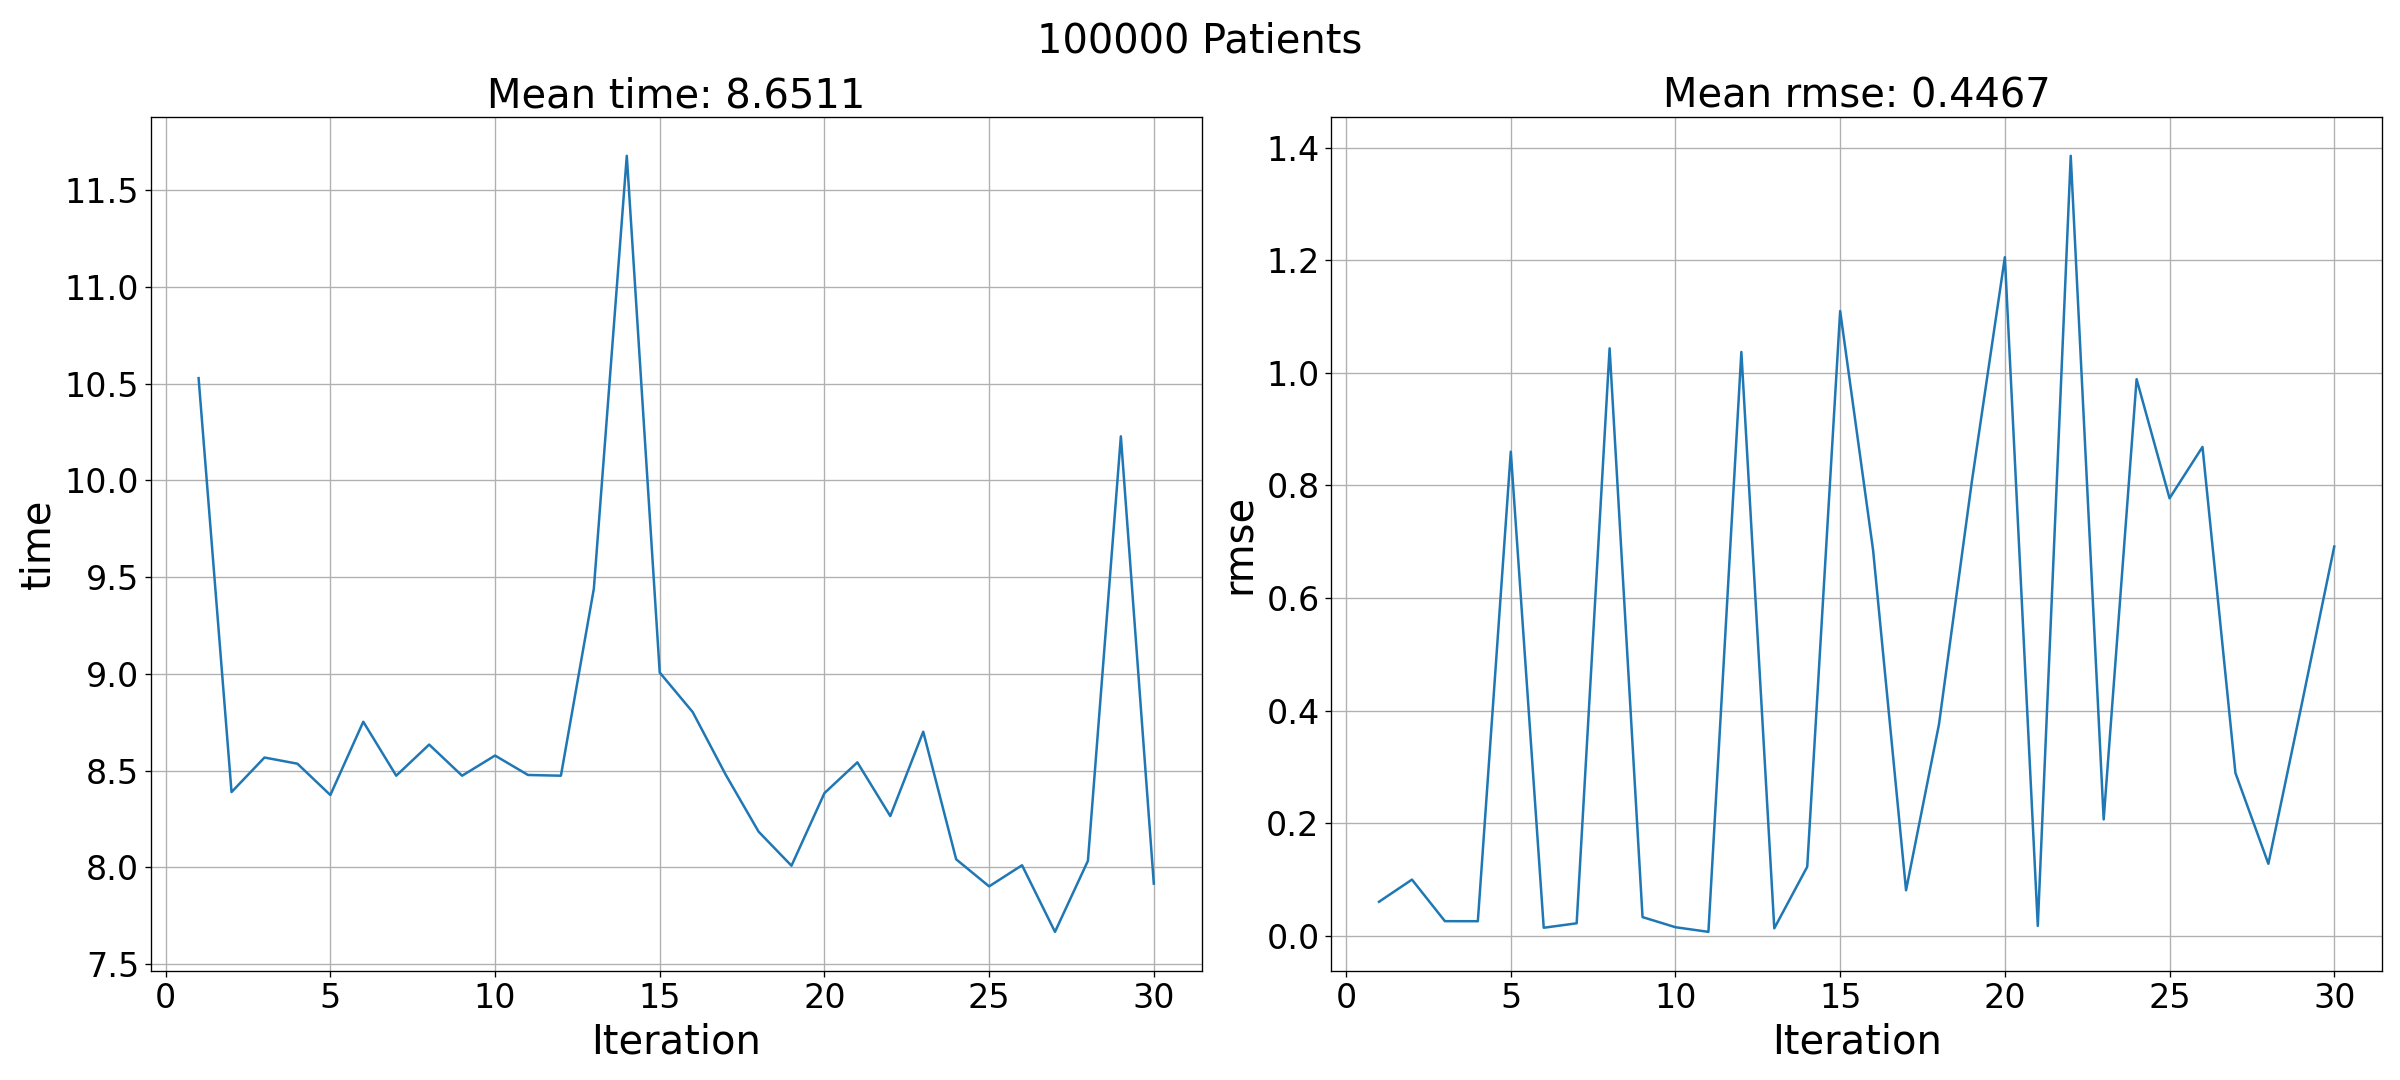
\includegraphics[width=\columnwidth]{../results/Stats/datasetB_100000_patients_rmse_and_time.png}
		\caption{RMSE and time for the external dataset.}
\end{figure}
\begin{figure}[h]
		\centering
		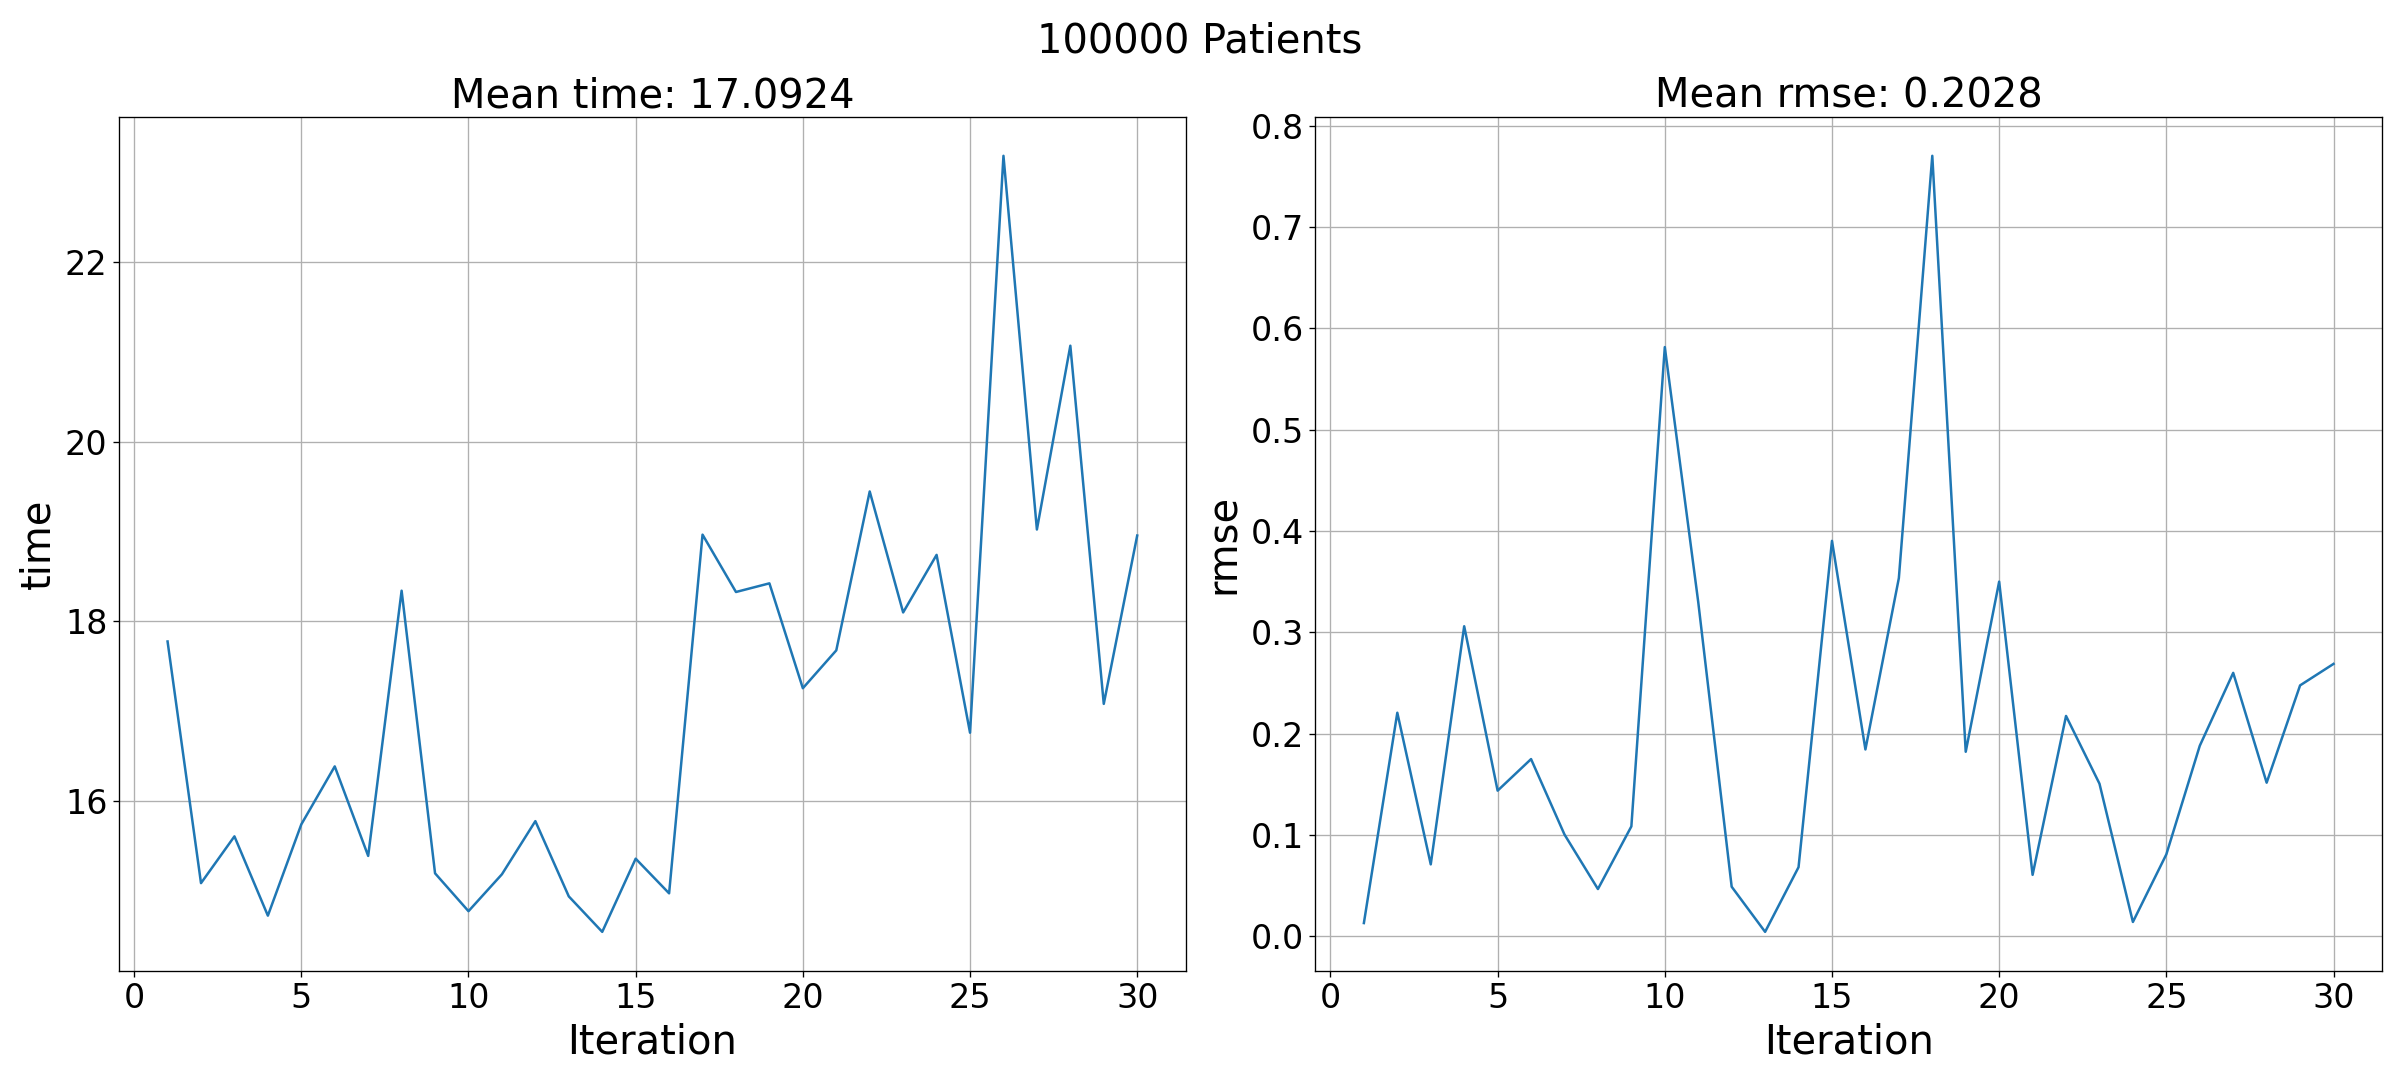
\includegraphics[width=\columnwidth]{../results/Stats/100k_patients_dataset_100000_patients_rmse_and_time.png}
		\caption{RMSE and time for the randomly filled dataset.}
\end{figure}
As it is possible to notice, for both datasets the recommendation system
presented the same jittery behaviour with a mean RMSE of 0.4467 for the
external dataset and 0.2028 for the randomly sampled one.
The difference in the average may be due to the random sample at test time.
Moreover the RMSE in the external dataset shows an higher mean value due to the
lower dimensionality of therapies available, while in the randomly
sampled one which has 204 dimensions the error influence may have a lower 
impact.
Regarding the execution time it is
possible to observe that in the external dataset the computation time
is halved with respect to the randomly generated one. This may be due to the
number of therapies available in the datasets, specifically 51 in the external
and 204 in the randomly filled one. The huge difference in the number
of therapies may have influenced negatively the time of computation due to
the vectors of ratings being 4 times bigger in the second dataset
increasing the computation time.
% Batches evalation
A second evaluation have been performed over the recommendation system aiming
to analyze its performances in function of the number of patients available.
In particular the analysis expoited four randomly filled dataset with 25, 50,
100 and 150 thousands patients.
\begin{figure}[h]
		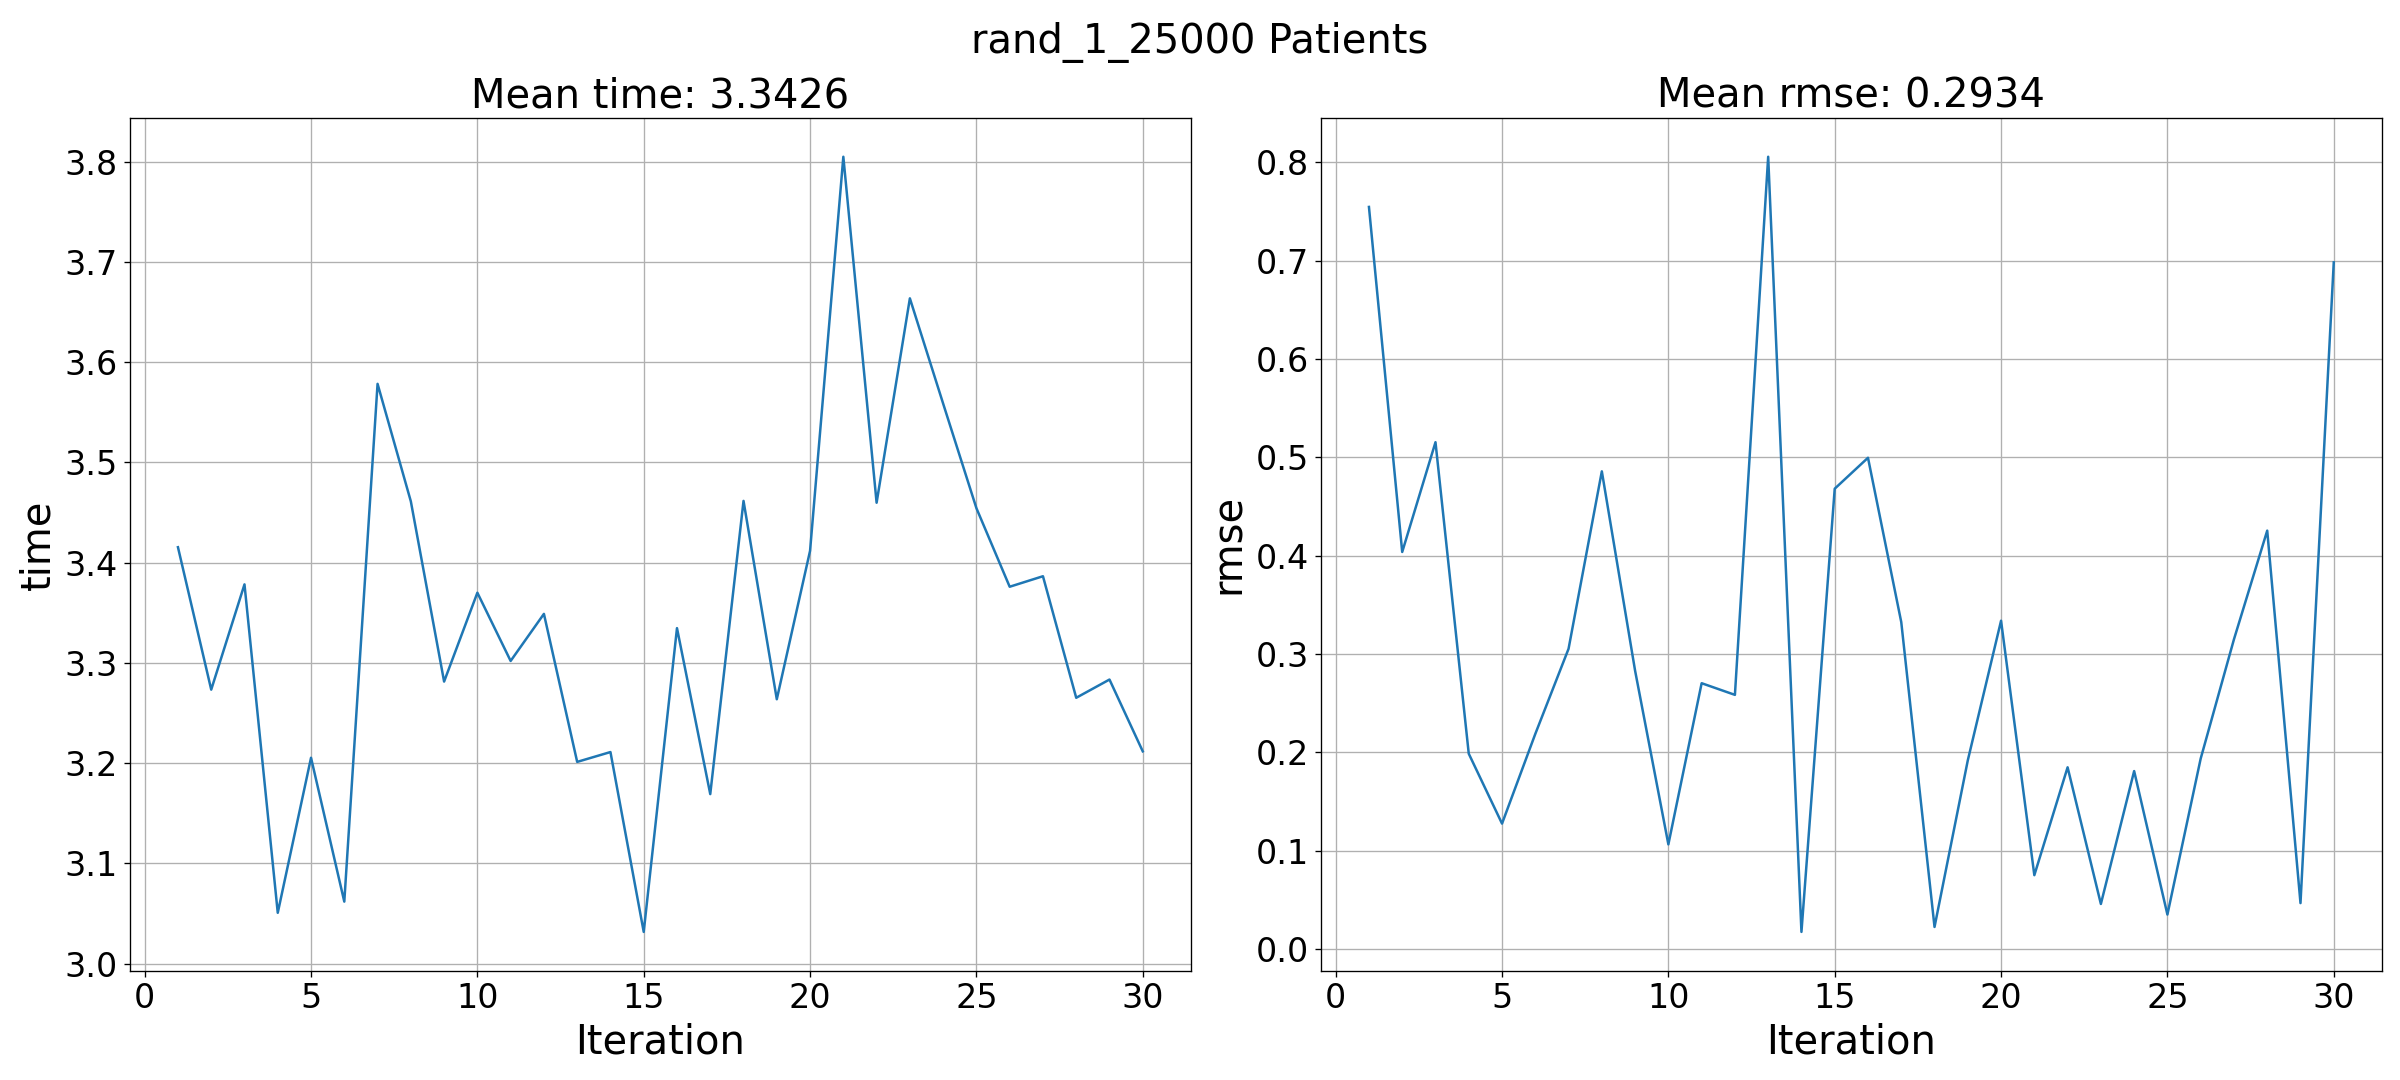
\includegraphics[width=\columnwidth]{../results/Stats/rand_1_25000_patients_rmse_and_time.png} \\
		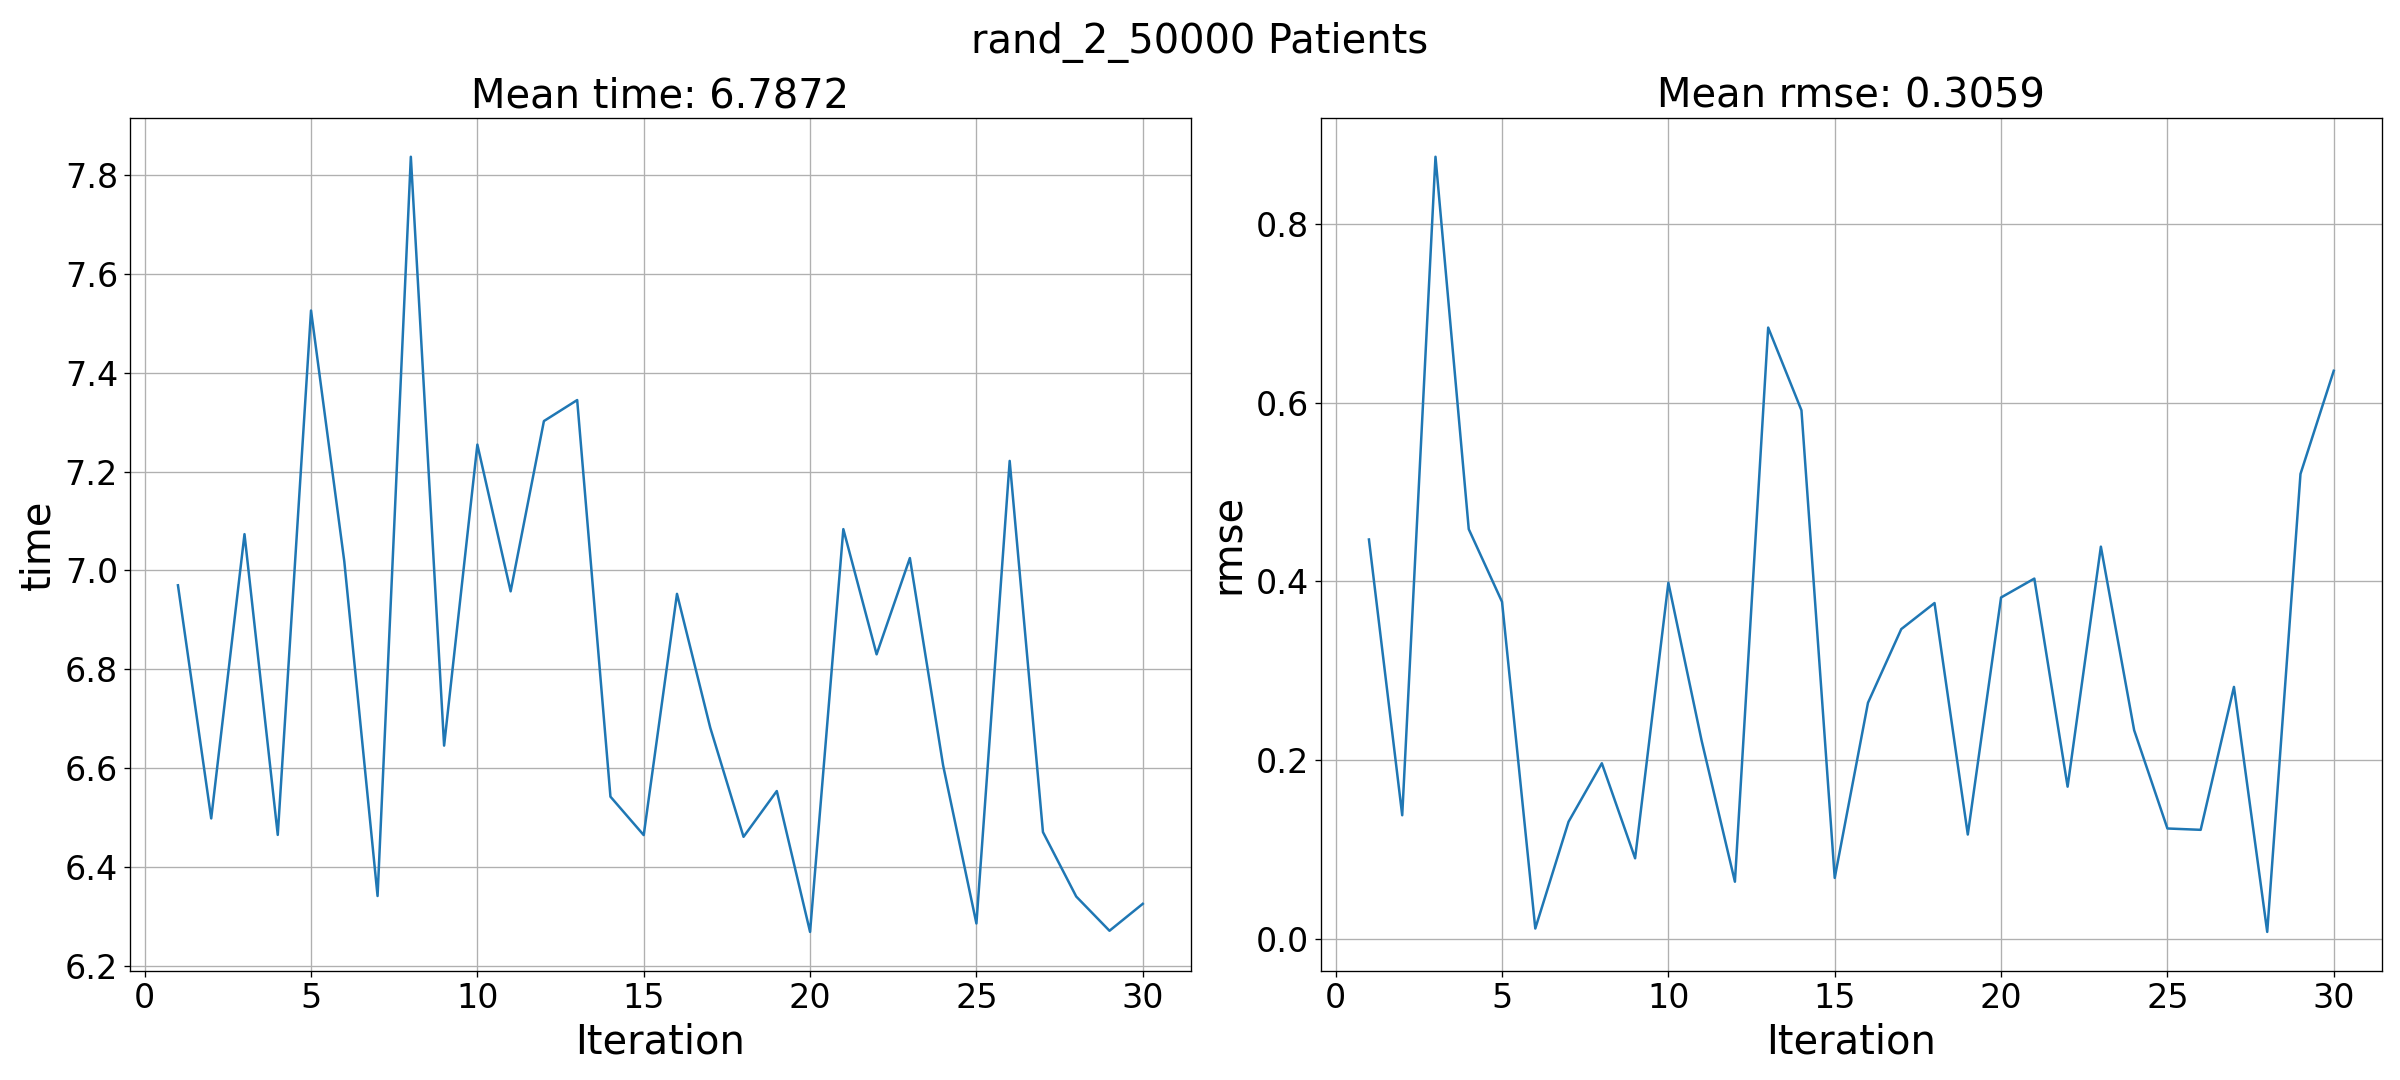
\includegraphics[width=\columnwidth]{../results/Stats/rand_2_50000_patients_rmse_and_time.png} \\
		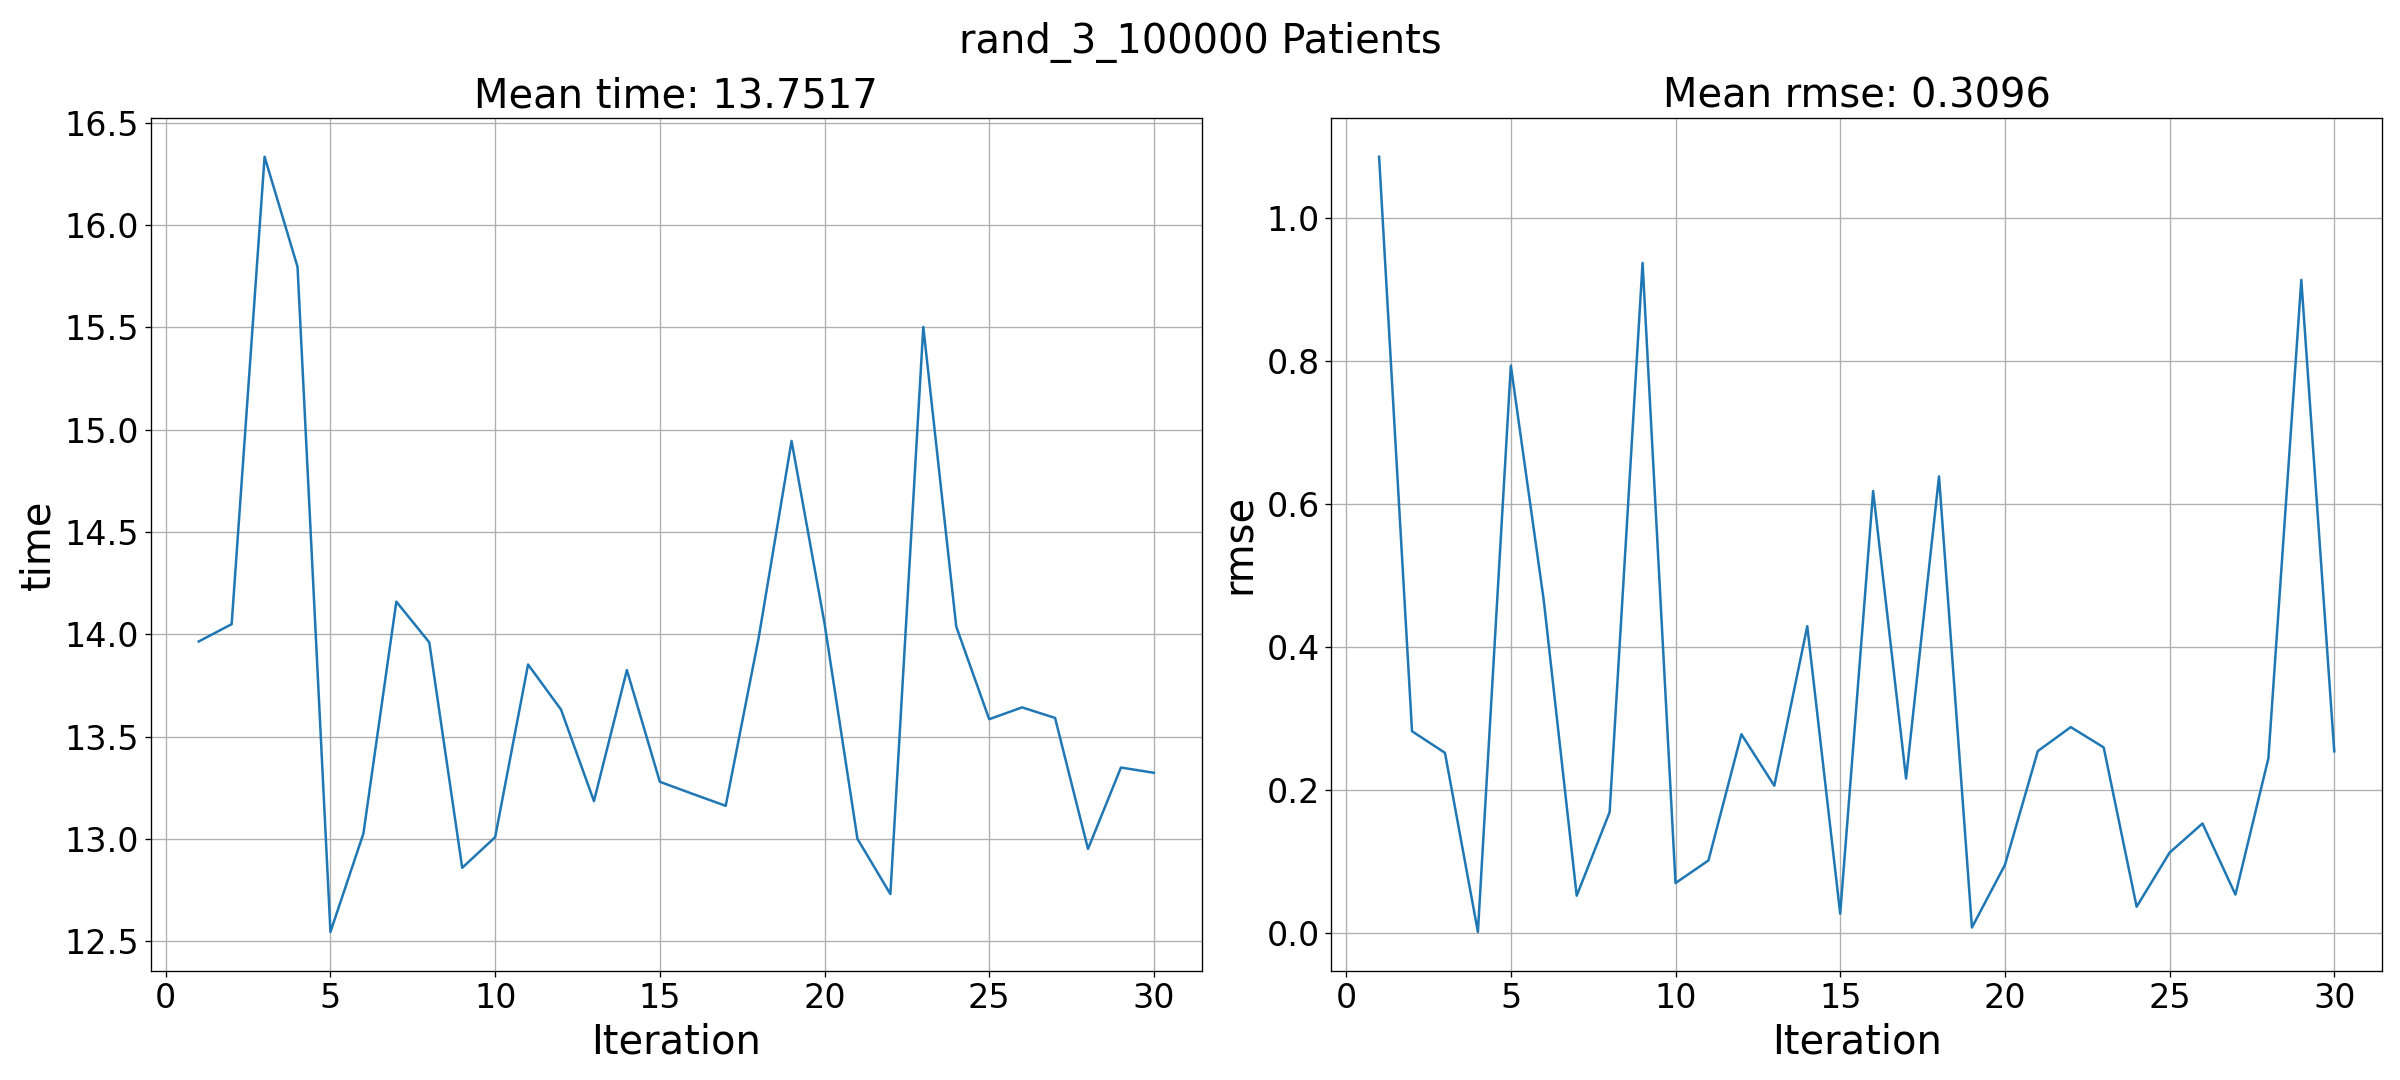
\includegraphics[width=\columnwidth]{../results/Stats/rand_3_100000_patients_rmse_and_time.png} \\
		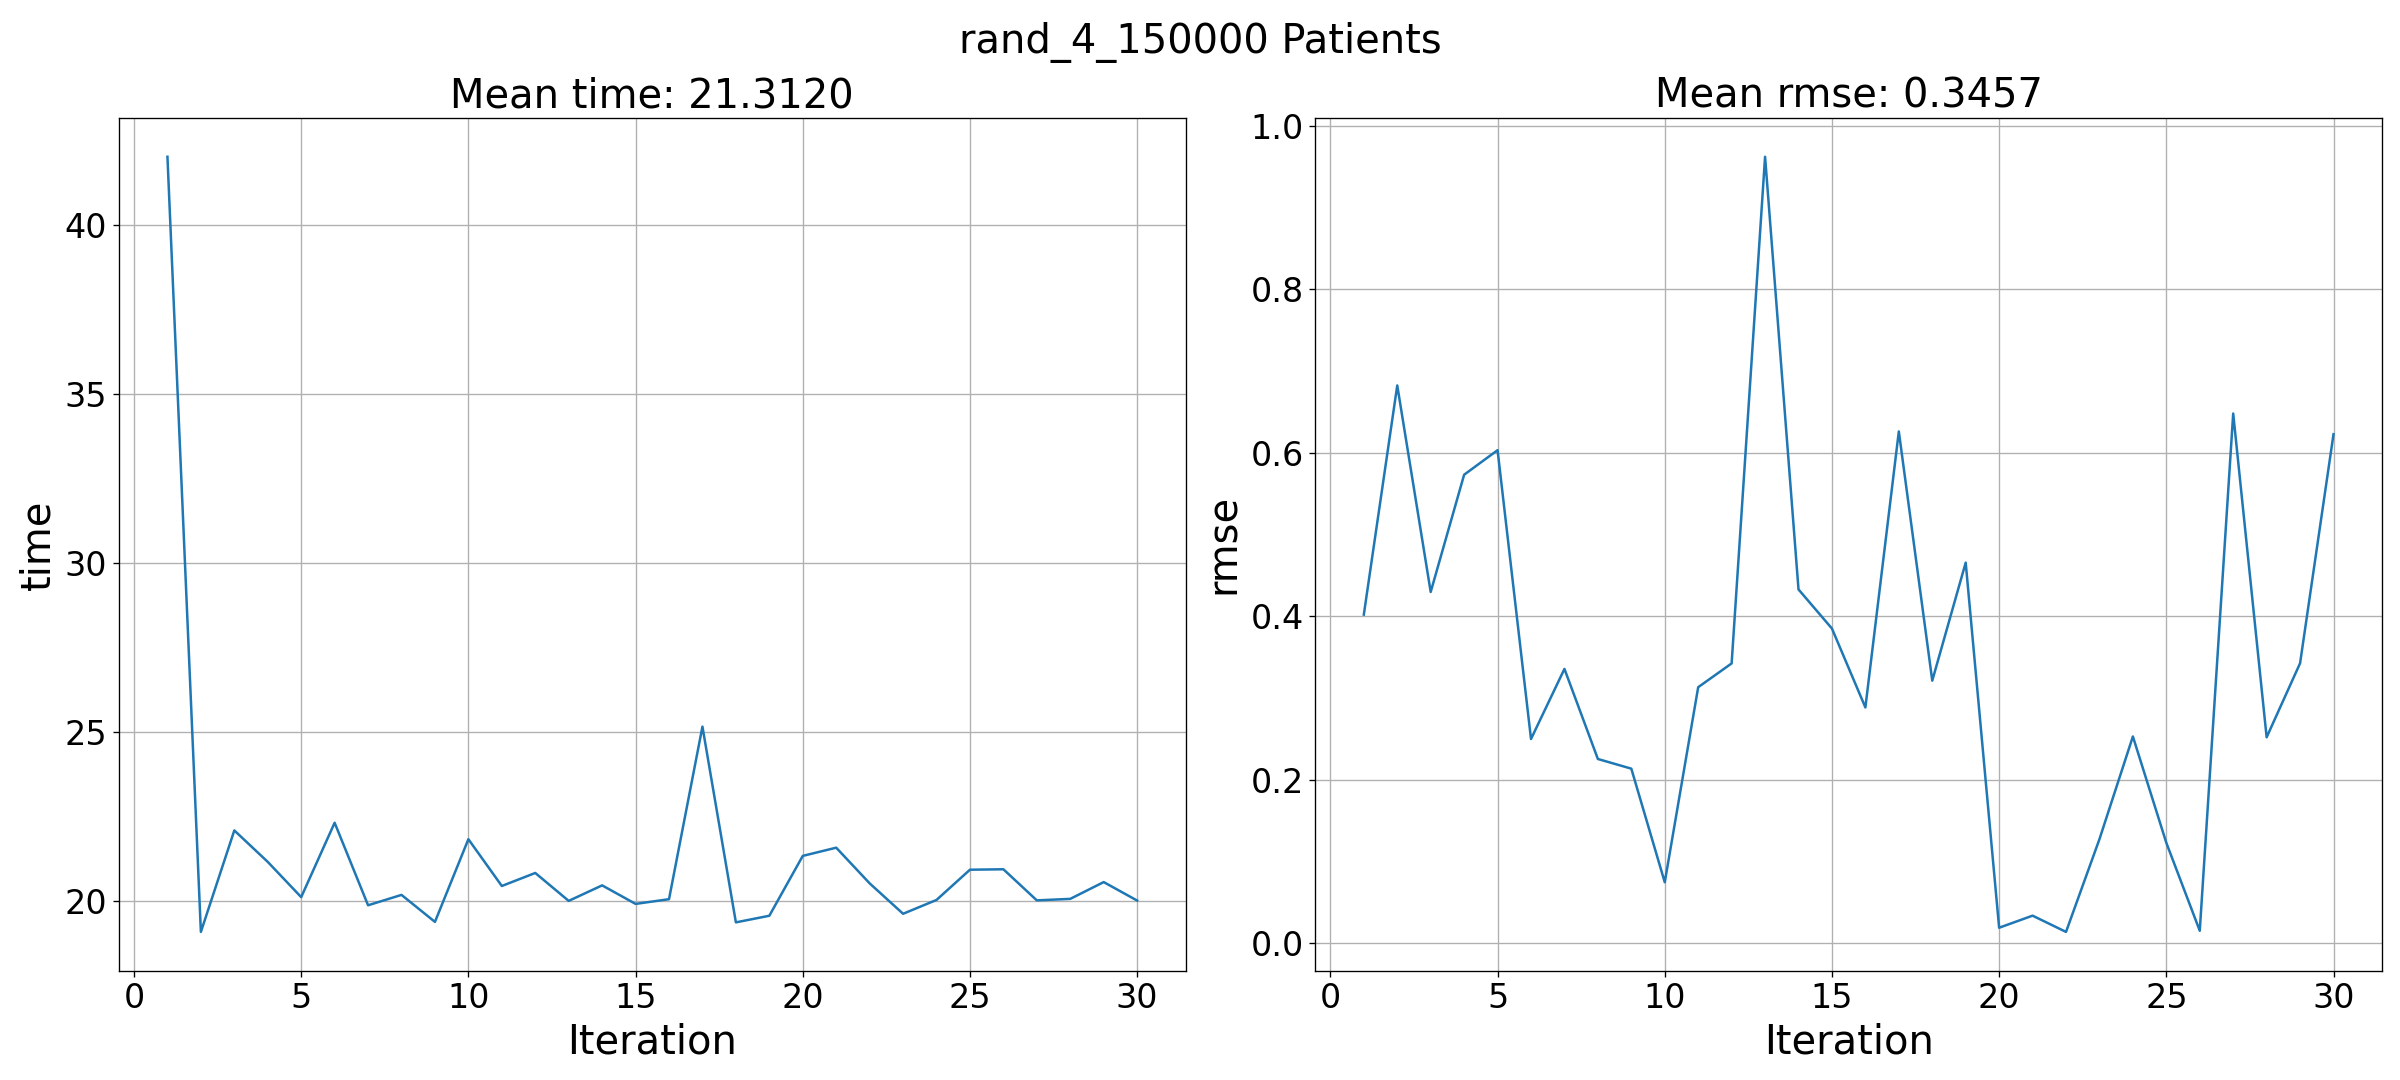
\includegraphics[width=\columnwidth]{../results/Stats/rand_4_150000_patients_rmse_and_time.png}
		\caption{Results of the recommendation system over four datasets having
				 25, 50, 100 and 150 thousands patients}
\end{figure}
\begin{figure}[h]
		\centering
		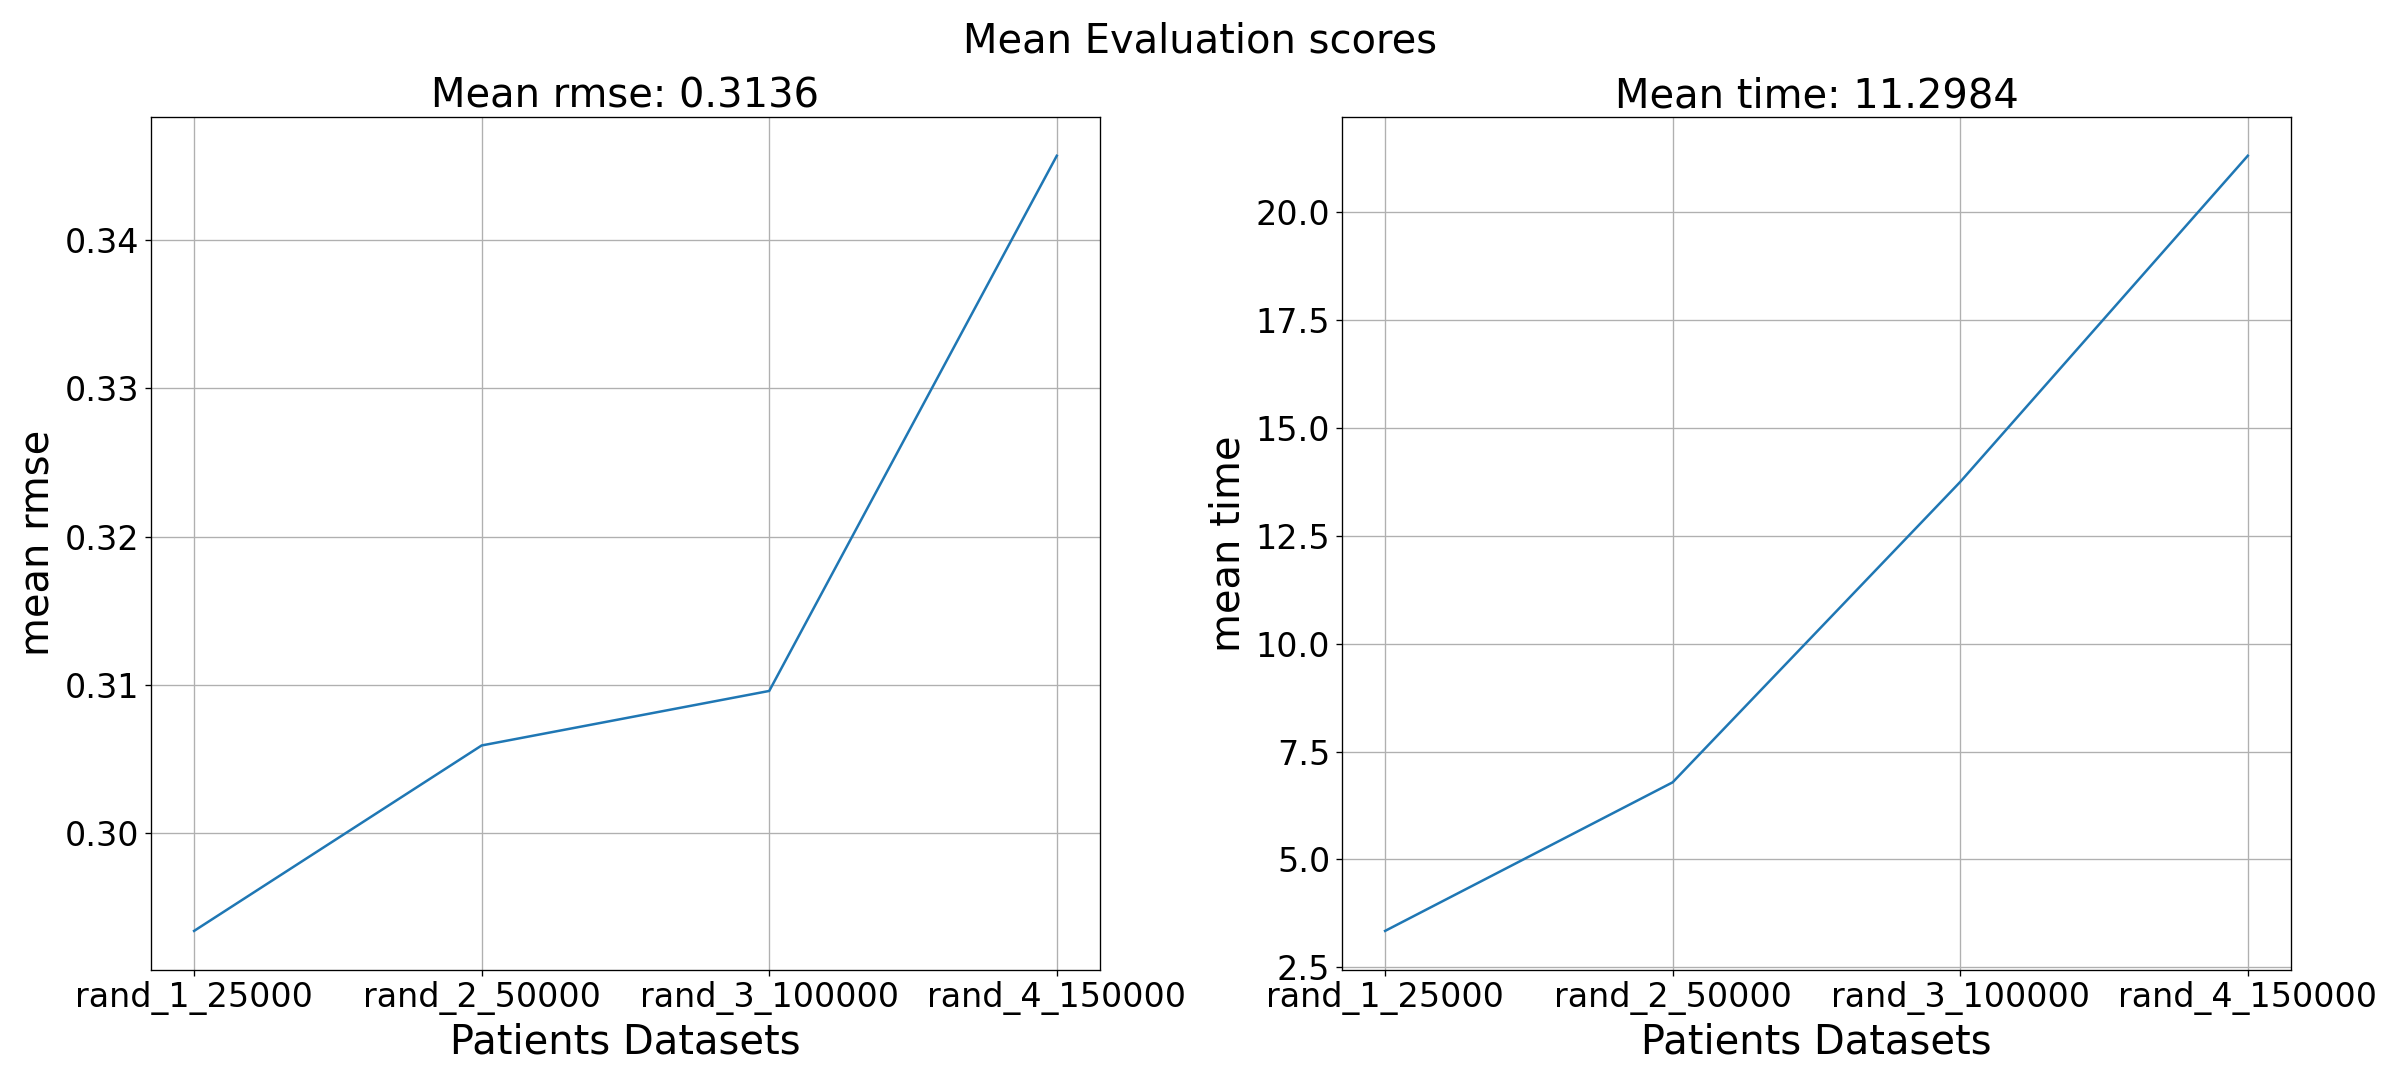
\includegraphics[width=\columnwidth]{../results/Stats/Evaluation_metrics_summary.png}
		\caption{Average RMSE and time scores for the four randomly filled
				 datasets.}
\end{figure}
\newpage
As it is possible to notice from figure 4, the RMSE value is subjected to the
stochasticity of the evaluation process and its values fluctuates, anyway it is
possible to assert that its mean value is, as the previous evaluations,
between
0.3136 with the highest peak at 0.35 and the lower one at 0.25.
Generally speaking the best and
worst cases may be seen as the extreme ones in which the worst is when the
patient had done nothing to cure its disease and so the recommendation system
resort to a content-base estimation, while the best one is when the patient
had done some trials to get rid of its sickness and the recommendation system
resort almost completely to the collaborative filtering component.
It is possible to notice a constant increase in the RMSE with the number of
patients in the dataset, anyway this behaviour may also be justified by the
random nature of the datasets.
About the time required by the system it is possible to infer a linearly
proportional dependency with the number of patients, possibly due to the bigger
utility matrix that has to be created for each disease to cure.
\clearpage
\bibliographystyle{ACM-Reference-Format}
\begin{thebibliography}{9}
		\bibitem{Pandas}
				https://pandas.pydata.org/
		\bibitem{ThPool}
				https://en.wikipedia.org/wiki/List\_of\_therapies
		\bibitem{CPool}
				https://www.nhsinform.scot/illnesses-and-conditions/a-to-z
		\bibitem{NamePool}
				https://github.com/philipperemy/name-dataset
\end{thebibliography}


%%
%% The next two lines define the bibliography style to be used, and
%% the bibliography file.
% \bibliographystyle{ACM-Reference-Format}
% \bibliography{sample-base}

%%
%% If your work has an appendix, this is the place to put it.
%% Please note that all the content must fit within the page limits, including any appendices.
%\appendix
%
%\section{Research Methods}
% ...

\end{document}
\endinput
